\documentclass[smaller,aspectratio=169]{beamer}
\mode<presentation>
{
  \usetheme[progressbar=frametitle]{metropolis}

  %\setbeamercovered{transparent}
}

% this is to use British English conventions
\usepackage[british]{babel}
% this is to include images/plots/etc
\usepackage{graphicx}
\graphicspath{{figures/}}
% this adds \footcite
\usepackage[backend=biber,style=authoryear,eprint=true, 
giveninits=true]{biblatex}
% this sets all maths fonts to the usual serif one
\usefonttheme[onlymath]{serif}
% this allows tikz graphics
\usepackage{tikz}
% externalize tikz to speed up compilation
%\usetikzlibrary{external}
%\tikzexternalize[prefix=cache/]
% this adds animations of tikz graphics (in suitable pdf viewers)
\usepackage[autoplay,loop,palindrome]{animate}
% this allows inclusion of standalone latex files
\usepackage{standalone}
% this allows more colours
\usepackage{xcolor}
\usepackage{amsmath}
\addbibresource{bibliography.bib}

%Customise \footcite command
\DeclareCiteCommand{\footcite}[\mkbibfootnote]
  {\usebibmacro{prenote}}
  {\printnames[family-given][-3]{labelname}%
   \newunit
   \printfield{archivePrefix}
   \printfield{eprint}
   %\printfield{primaryClass}%
   \newunit
   \printlabeldateextra}
  {\addsemicolon\space}
  {\usebibmacro{postnote}}
  
\newcommand{\rad}{\mathrm{rad}}
\newcommand{\tl}{\tilde{\ell}}
\newcommand{\tm}{\tilde{m}}
\newcommand{\rmd}{\mathrm{d}}

\title[Eccentric Kicks] % (optional, use only with long paper titles)
{Kicks from Eccentric Black Hole Binaries}

%\subtitle
%{Include Only If Paper Has a Subtitle}

\author{
    \textbf{Miren~Radia}\textsuperscript{{1}} \and 
    Ulrich~Sperhake\textsuperscript{1} \and 
    Emanuele~Berti\textsuperscript{2} \and 
    Robin~Croft\textsuperscript{1}}

\institute
{
    \textsuperscript{1} Department of Applied Mathematics \& 
    Theoretical Physics, University of Cambridge\\
    \textsuperscript{2} Department of Physics \& Astronomy, 
    Johns Hopkins University
}

\date{GRChombo Meeting: 14 Dec 2020}
% - Either use conference name or its abbreviation.
% - Not really informative to the audience, more for people (including
%   yourself) who are reading the slides online

\subject{Numerical Relativity}
% This is only inserted into the PDF information catalog. Can be left
% out.

% Uncomment \logo and comment \titlegraphic to put University logo on every page
%\logo{
\includegraphics[height=0.5cm]{uni-cam-logo}\hspace{1 cm}}
\titlegraphic{
    \vspace{6 cm}
    
\includegraphics[width=2cm]{grchombo-logo.png}
    \hfill
    
\includegraphics[width=3cm]{uni-cam-logo.eps}
    }

% Delete this, if you do not want the table of contents to pop up at
% the beginning of each subsection:
% \AtBeginSubsection[]
% {
%   \begin{frame}<beamer>{Outline}
%     \tableofcontents[currentsection,currentsubsection]
%   \end{frame}
% }


% If you wish to uncover everything in a step-wise fashion, uncomment
% the following command: 

\beamerdefaultoverlayspecification{<+->}


\begin{document}

\begin{frame}
  \titlepage
\end{frame}

\begin{frame}{Outline}
  \tableofcontents
  % You might wish to add the option [pausesections]
\end{frame}


% Structuring a talk is a difficult task and the following structure
% may not be suitable. Here are some rules that apply for this
% solution: 

% - Exactly two or three sections (other than the summary).
% - At *most* three subsections per section.
% - Talk about 30s to 2min per frame. So there should be between about
%   15 and 30 frames, all told.

% - A conference audience is likely to know very little of what you
%   are going to talk about. So *simplify*!
% - In a 20min talk, getting the main ideas across is hard
%   enough. Leave out details, even if it means being less precise than
%   you think necessary.
% - If you omit details that are vital to the proof/implementation,
%   just say so once. Everybody will be happy with that.

\section{Introduction}

\begin{frame}{What are kicks?}
    \begin{itemize}
        \item 
            \alert{Anisotropic} emission of GWs will carry a net linear momentum.
        \item
            Conservation of momentum means a recoil (or \alert{kick}) 
            is imparted to the emitting system.
        \item
            For binary BH mergers, the necessary \alert{asymmetry} can be 
            e.g. unequal masses or misaligned spins.
        \item
            Astrophysical consequences: compare kick velocity $v$ with escape 
            velocity $v_{\text{esc}}$ of various astrophysical environments
            \begin{itemize}
                \item 
                    Globular clusters: $v_{\text{esc}}=\mathcal{O}(10\text{ km/s})$,
                    quasicircular non-spinning BBH mergers: $v = \mathcal{O}(100\text{ km/s})$.
                \item
                    Can use kicks to constrain growth theories of 
                    SMBHs at the centre of dark matter halos.
            \end{itemize}
    \end{itemize}
\end{frame}


\begin{frame}{Why consider eccentricity?}
    \begin{itemize}
        \item 
            We still don't know how BH binaries form 
            (there are several suggested \alert{formation channels})!
        \item
            For \alert{isolated binary} systems, GW emission acts to 
            circularize orbits.
        \item
            Orbital Eccentricity expected to be a distinguishing feature of 
            \alert{dynamical} formation channels in e.g. globular 
            clusters, galactic nuclei, etc.
        \item
            No evidence from LIGO O1 and O2 runs\footcite{Salemi:2019owp} 
            but GW190521 is potentially consistent with\footcite{Gayathri:2020coq} 
            $e\simeq0.7$.
        \item
            Also just another way to possibly accentuate asymmetry.
    \end{itemize}
\end{frame}

\section{Setup and Methods}

\subsection{BH binary configurations}
\begin{frame}{BH binary configurations}
	\begin{center}
    \resizebox{0.7\textwidth}{!}{
    \only<3->{
	    \begin{animateinline}{10}
	    \multiframe{60}{rd = 6+0.1}{
	        \begin{tikzpicture}
	        	% background to ensure constant size
	        	\draw[fill=black!2,color=black!2] (-9,-1.2) rectangle (5,2);
	        	
	        	\node at (-2,2) {$E_{\text{b}}=M_{\text{ADM}}-(M_1+M_2)=\text{const.}$};
	
	        	% line connecting BHs
	        	\draw[dashed] (-2*\rd/3,0) -- (\rd/3,0);
	        	\filldraw[color=white, fill=red] (0,0) circle (0.05);
	        
	        	% small BH
	        	\filldraw[fill = black] (-2*\rd/3,0) circle (0.3);
	        	\draw[very thick,-latex, color=black] (-2*\rd/3,0) -- (-2*\rd/3,4/3-16/\rd);
	        	\node[anchor=west, color=black] at (-2*\rd/3,4/3-16/\rd) {$p$};
	        	\node[color=white] at (-2*\rd/3,0) {$M_1$};
	        	
	        	% big BH
	        	\filldraw[fill = black] (\rd/3,0) circle (0.6);
	        	\draw[very thick,-latex, color=black] (\rd/3,0) -- (\rd/3,0.3-4/3+16/\rd);
	        	\node[anchor=east, color=black] at (\rd/3,0.3-4/3+16/\rd) {$p$};
	        	\node[color=white] at (\rd/3,0) {$M_2$};
	        
	        	% length
	        	\draw[dotted] (\rd/3,0) -- (\rd/3,-1.2);
	        	\draw[dotted] (-2*\rd/3,0) -- (-2*\rd/3,-1.2);
	        	\draw[latex-latex] (-2*\rd/3,-1) -- (\rd/3,-1);
	        	\node[anchor=south] at (-\rd/6,-1.5) {$D$};
	        	
	        	% axes
	        	\draw[-latex] (0,0) -- (0,1);
	        	\node [anchor=east] at (0,1) {$y$};
	        	\draw[-latex] (0,0) -- (1,0);
	        	\node[anchor=north] at (1,0) {$x$};
	        \end{tikzpicture}
	    }
	    \end{animateinline}
    }
	\only<-2>{
  		\begin{animateinline}{1}
		\multiframe{1}{rd = 6+0.1}{
			\begin{tikzpicture}
			% background to ensure constant size
			\draw[fill=black!2,color=black!2] (-9,-1.2) rectangle (5,2);
			
			\node at (-2,2) {$E_{\text{b}}=M_{\text{ADM}}-(M_1+M_2)=\text{const.}$};
			
			% line connecting BHs
			\draw[dashed] (-2*\rd/3,0) -- (\rd/3,0);
			\filldraw[color=white, fill=red] (0,0) circle (0.05);
			
			% small BH
			\filldraw[fill = black] (-2*\rd/3,0) circle (0.3);
			\draw[very thick,-latex, color=black] (-2*\rd/3,0) -- (-2*\rd/3,4/3-16/\rd);
			\node[anchor=west, color=black] at (-2*\rd/3,4/3-16/\rd) {$p$};
			\node[color=white] at (-2*\rd/3,0) {$M_1$};
			
			% big BH
			\filldraw[fill = black] (\rd/3,0) circle (0.6);
			\draw[very thick,-latex, color=black] (\rd/3,0) -- (\rd/3,0.3-4/3+16/\rd);
			\node[anchor=east, color=black] at (\rd/3,0.3-4/3+16/\rd) {$p$};
			\node[color=white] at (\rd/3,0) {$M_2$};
			
			% length
			\draw[dotted] (\rd/3,0) -- (\rd/3,-1.2);
			\draw[dotted] (-2*\rd/3,0) -- (-2*\rd/3,-1.2);
			\draw[latex-latex] (-2*\rd/3,-1) -- (\rd/3,-1);
			\node[anchor=south] at (-\rd/6,-1.5) {$D$};
			
			% axes
			\draw[-latex] (0,0) -- (0,1);
			\node [anchor=east] at (0,1) {$y$};
			\draw[-latex] (0,0) -- (1,0);
			\node[anchor=north] at (1,0) {$x$};
			\end{tikzpicture}
		}
		\end{animateinline}
	}
	}
	\end{center}

    \begin{itemize}
        \item<1->
            We consider \alert{four sequences} (\texttt{sq2:3}, \texttt{sq1:2}, 
            \texttt{lq1:2} and \texttt{sq1:3}) with \alert{three different 
            mass ratios}: $q=2/3$, $1/2$ and $1/3$\footnote{
            Maximum kick in quasicircular case occurs at $q\simeq1/2.77$.}.
        \item<2->
            Two sequences for $q=1/2$, one longer\footnote{In the quasicircular limit: short sequence configurations do $\sim3$ orbits and long $\sim6$ orbits} to identify any 
            possible artifacts due to short inspiral phases.
        \item<3->
            No well-defined notion of eccentricity in full GR, 
            so we use an estimate coming from 
            PN theory\footcite{Memmesheimer:2004cv}: 
            $e_t$ (in harmonic coordinates).
    \end{itemize}
	\vskip 0.5em
\end{frame}

\subsection{Numerical methods}
\begin{frame}{Numerical methods}
    \begin{itemize}
        \item 
            \textsc{GRChombo} was used with \alert{CCZ4} for 
            \texttt{sq2:3} and \texttt{sq1:3}.
            \begin{itemize}
                \item 
                    Used new \alert{sixth order spatial derivatives} code 
                    - necessary for sufficient phase accuracy.
                \item
                    Quite a bit of work to get tagging criterion to a satisfactory
                    state for accurate BH evolution (cf. horizon area 
                    drift issues).\footnote{Thanks to 
                    Katy for her work on this last year.}
            \end{itemize}
        \item
            \textsc{Lean} was used with \alert{BSSN} for \texttt{sq1:2} and \texttt{lq1:2}.
        \item
            Both codes used the \texttt{TwoPunctures}\footcite{Ansorg:2004ds} 
            spectral solver for \alert{Bowen-York puncture} initial data
            \begin{itemize}
                \item 
                    I have integrated this into GRChombo - might be useful 
                    to get this into the public code?
            \end{itemize}
    \end{itemize}
\end{frame}

\subsection{Diagnostic quantities}
\begin{frame}{Diagnostic quantities}
	\begin{itemize}
		\item 
			Radiated energy $E^{\rad}$, 
			linear momentum $\mathbf{P}^{\rad}$ and 
			angular momentum $\mathbf{J}^{\rad}$ computed \alert{directly} 
			from extracted $\Psi_4$ values on extraction spheres e.g.
			\begin{equation}
				\mathbf{P}^{\rad}(t) = \lim_{r\to\infty}\frac{r^2}{16\pi}
				\int_{t_0}^t\rmd t^\prime\oint_{S^2_r}\rmd\Omega\,
				\hat{\mathbf{e}}_r\left|\int_{-\infty}^{t^\prime}\rmd t^{\prime\prime}\,
				\Psi_4\right|^2.
				\label{eq:Prad}
			\end{equation}
		\item
			Kick obtained from $\mathbf{v}=-\mathbf{P}^{\rad}/M_{\text{fin}}$.
		\item
			Also computed\footnote{By symmetry $P^\rad_z=0$.} 
			$\mathbf{P}^{\rad}$
			from multipolar amplitudes of $\Psi_4=\sum_{\ell,m}\psi_{\ell,m}\left[{}_{-2}Y^{\ell,m}\right]$:
			\begin{multline}
				P_+(t) = P^\rad_x(t) + \mathrm{i}P^\rad_y(t)
				 = \lim_{r\to\infty}\frac{r^2}{8\pi}\sum_{\tl=2}^{\infty}
				 \sum_{\tm=-\tl}^{\tl}\int_{t_0}^t\rmd t^{\prime}
				\left\{\left(\int^{t^\prime}_{-\infty}\rmd t^{\prime\prime}\, 
				\psi_{\tl,\tm}\right)\right.\\
				\left.\times\left(\int_{-\infty}^{t^\prime} 
				\left[a_{\tl,\tm}\bar{\psi}_{\tl,\tm+1}+ 
				b_{\tl,-\tm}\bar{\psi}_{\tl-1,\tm+1}-
				b_{\tl+1,\tm+1}\bar{\psi}_{\tl+1,\tm+1}\right]
				\rmd t^{\prime\prime}\right)\right\},
				\label{eq:P+rad}
			\end{multline}
			\vspace{0.5 em}
	\end{itemize}

\end{frame}

\subsection{Numerical accuracy}
\begin{frame}{Convergence and comparison with \textsc{Lean}}
    \includegraphics[width=0.45\linewidth]{grchombo-convergence4.eps}
    \hfill
    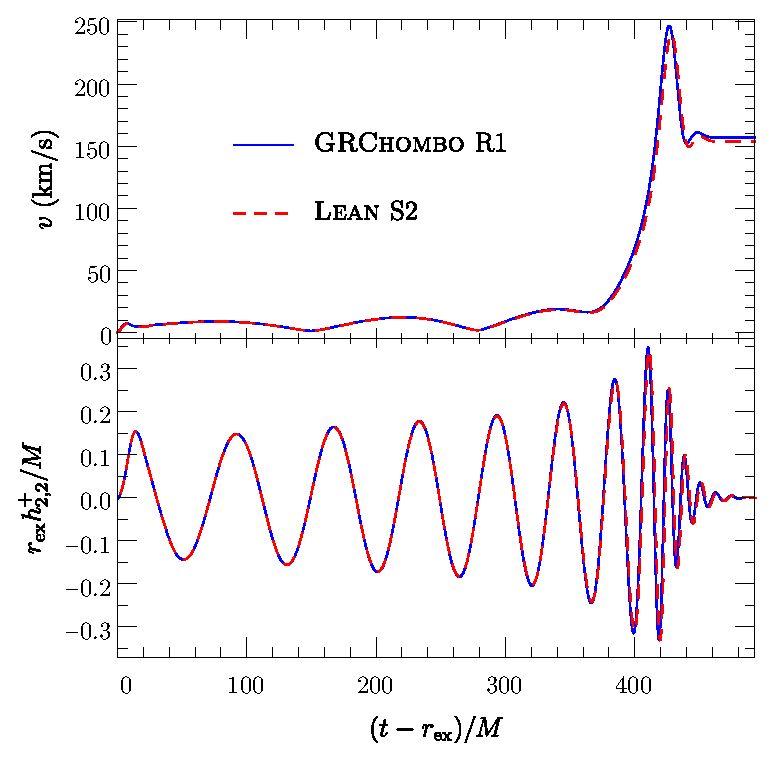
\includegraphics[width=0.45\linewidth]{grchombo-lean-comparison3.eps}
\end{frame}

\section{Results}

\subsection{Recoil velocity, radiated energy and final spin}
\begin{frame}{Recoil velocity, radiated energy and final spin}
    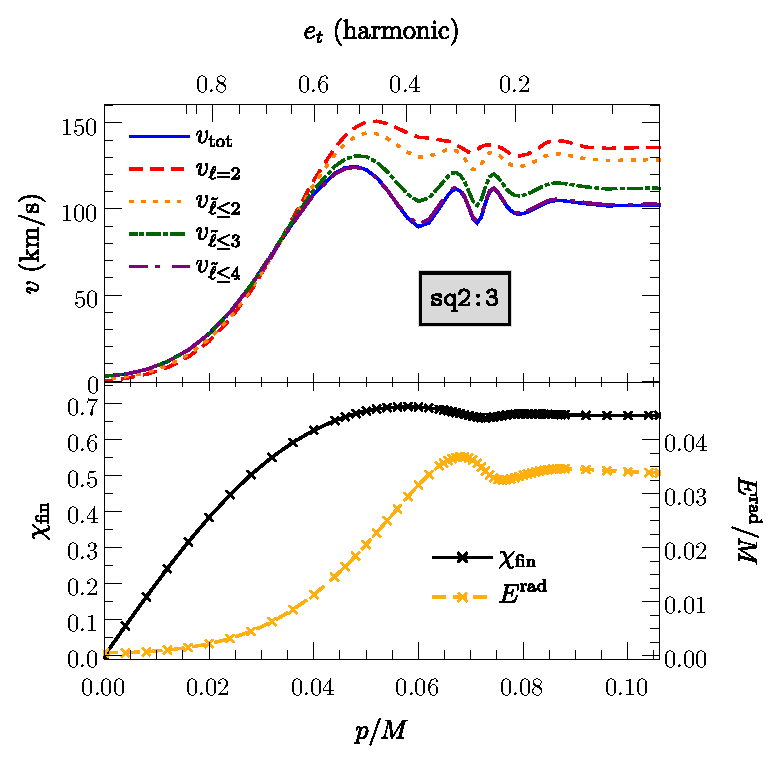
\includegraphics[width=0.45\linewidth]{kick-q1.5-wlabel.eps}
    \hfill
    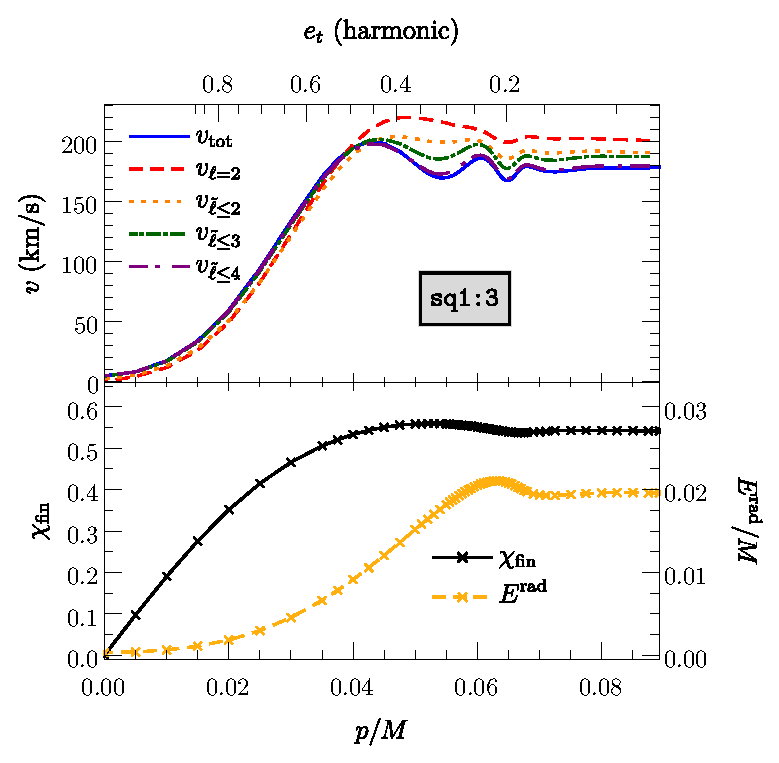
\includegraphics[width=0.45\linewidth]{kick-q3-wlabel.eps}
\end{frame}

\begin{frame}{Recoil velocity, radiated energy and final spin}
	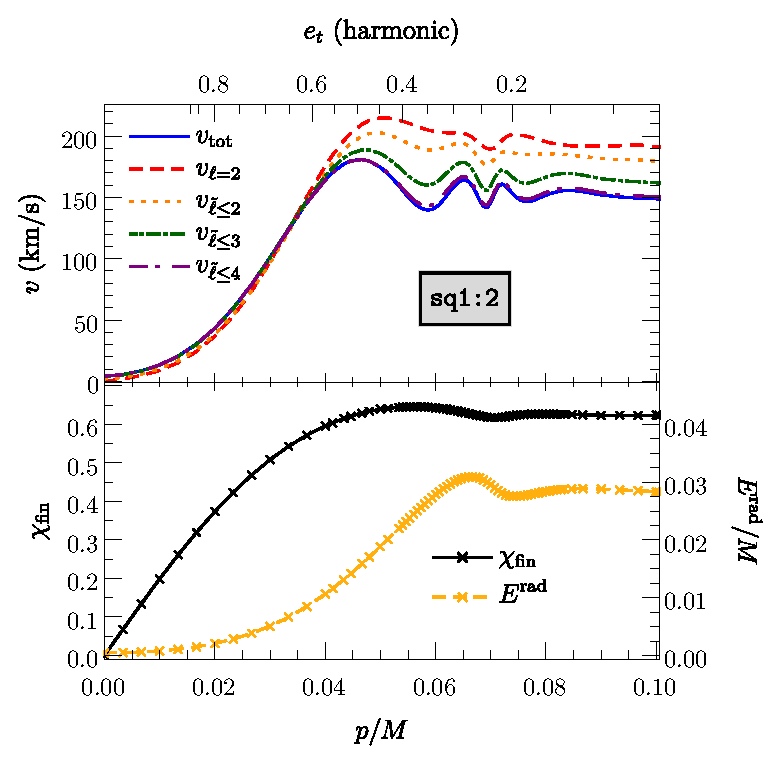
\includegraphics[width=0.45\linewidth]{kick-q2-wlabel.eps}
	\hfill
	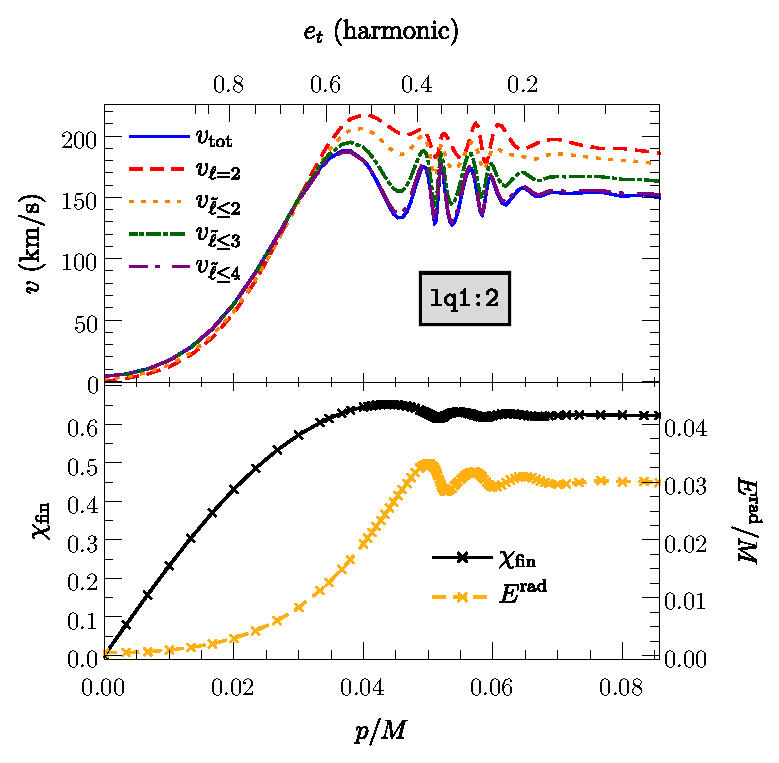
\includegraphics[width=0.45\linewidth]{kick-q2l-wlabel.eps}
\end{frame}

\begin{frame}{Observations}
	\begin{columns}
		\column{0.4\textwidth}
			\centering
			\only<.->{
				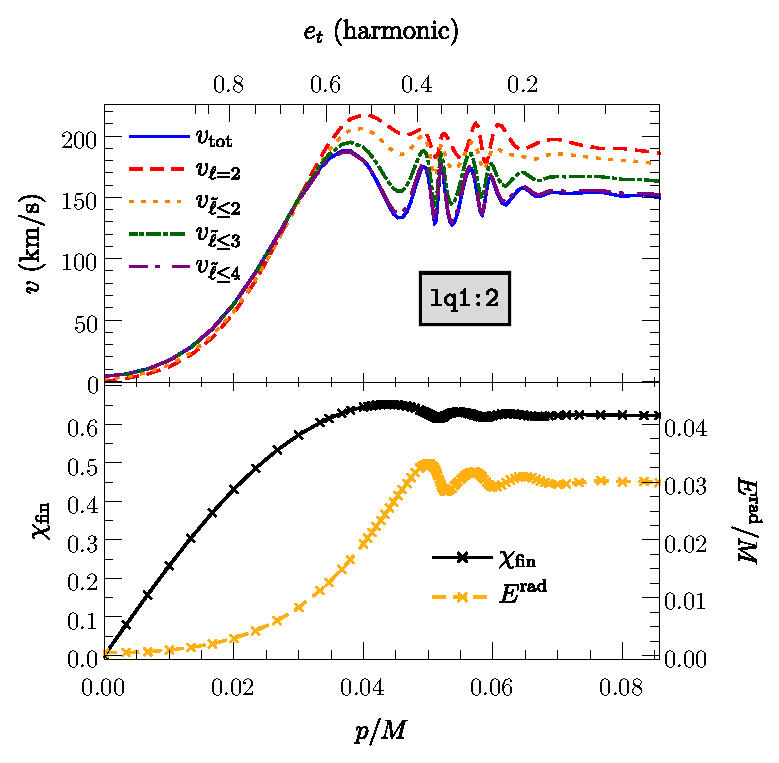
\includegraphics[width=\columnwidth]{kick-q2l-wlabel.eps}
			}
		\column{0.6\textwidth}
			\begin{itemize}
				\item<.-> 
					\alert{Maximum} kick occurs at $e\sim0.5$ and 
					is about 22/22/25/12\% larger than the 
					quasicircular value for 
					\texttt{sq2:3}/\texttt{sq1:2}/\texttt{lq1:2}/\texttt{sq1:3}.
				\item
					\alert{Oscillatory} behaviour in $v=v(p)$ 
					which increases in 
					frequency and amplitude for longer inspirals. 
					If this pattern continues,
					we would expect the kick to depend 
					\alert{highly sensitively} for even longer inspirals
				\item
					Fewer/less pronounced oscillations in radiated 
					energy/final spin with different extrema.
				\item
					Oscillations present in all considered partial 
					sums of Eq.~\eqref{eq:P+rad},
					albeit somewhat less pronounced.
				\item
					Higher-order terms with $\tl>2$ \alert{decrease} the kick.
			\end{itemize}
	\end{columns}
\end{frame}

\subsection{Kick angle}
\begin{frame}{Kick angle}
	\begin{columns}
		\column{0.6\textwidth}
			\begin{itemize}
				\item<.->
					Only ``special'' direction is the \alert{apoapsis}.
				\item<+->
					Want to look at \alert{infall direction} 
					relative to apoapsis.
				\item<+-> 
					No good definition of infall direction so 
					use \alert{kick angle}:
					\begin{equation}
					\vartheta = \text{arg}(v_x + \mathrm{i}v_y).
					\end{equation}
			\end{itemize}
			\centering
			\only<-.>{\vspace{0.5\textheight}}
			\only<+->{
			\resizebox{!}{0.5\textheight}
			{
				%\tikzexternaldisable
				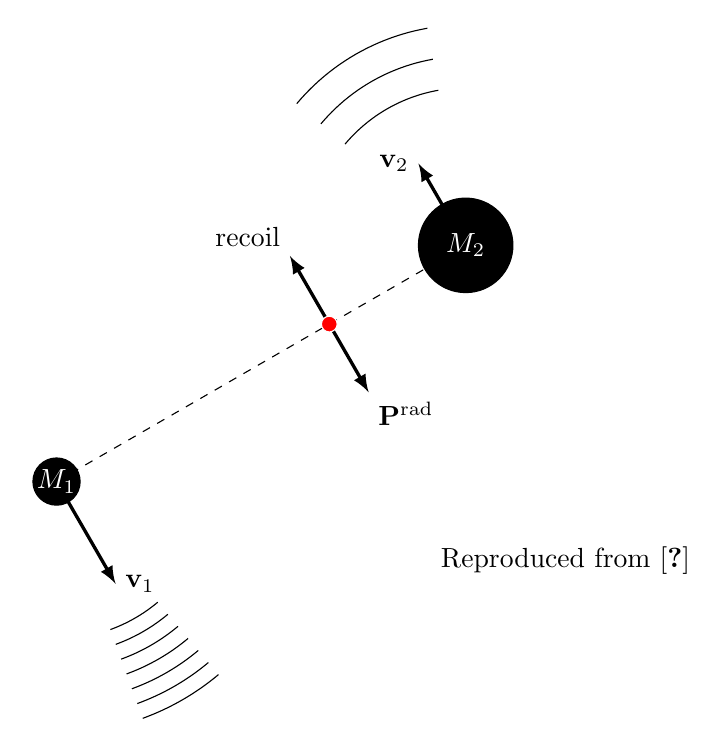
\begin{tikzpicture}
					% line connecting BHs
					\draw[dashed] (-3.46410161514,-2) -- (1.73205080757,1);
					
					% small BH
					\filldraw[fill = black] (-3.46410161514,-2) circle (0.3);
					\draw[very thick,-latex] (-3.46410161514,-2) -- 
					(-2.71410161514,-3.29903810568);
					\node[anchor=west] at (-2.71410161514,-3.29903810568) {$\mathbf{v}_1$};
					\node[color=white] at (-3.46410161514,-2)  {$M_1$};
					\foreach \r in {2,2.2,2.4,2.6,2.8,3,3.2}
					\draw[domain=-70:-50,smooth] plot 
					({-3.46410161514 + \r*cos(\x)},{-2+\r*sin(\x)});
					
					% big BH
					\filldraw[fill = black] (1.73205080757,1) circle (0.6);
					\draw[very thick,-latex] (1.73205080757,1) -- 
					(1.13205080757,2.03923048454);
					\node[anchor=east] at (1.13205080757,2.03923048454) {$\mathbf{v}_2$};
					\node[color=white] at (1.73205080757,1) {$M_2$};
					\foreach \r in {2,2.4,2.8}
					\draw[domain=140:100] plot 
					({1.73205080757+ \r*cos(\x)},{1+\r*sin(\x)});
					
					% centre of mass
					\draw[very thick,-latex] (0,0) -- (0.5,-0.86602540378);
					\node[anchor=north west] at (0.5,-0.86602540378) 
					{$\mathbf{P}^{\mathrm{rad}}$};
					\draw[very thick,-latex] (0,0) -- (-0.5,0.86602540378);
					\node[anchor=south east] at (-0.5,0.86602540378) {$\text{recoil}$};
					
					\filldraw[color=white, fill=red] (0,0) circle (0.1);
					
					\node at (3,-3) {Reproduced from \cite{Wiseman:1992dv}};
				\end{tikzpicture}
				%\tikzexternalenable
		}
		}
		\column{0.4\textwidth}
			\only<-.>{
				\vphantom{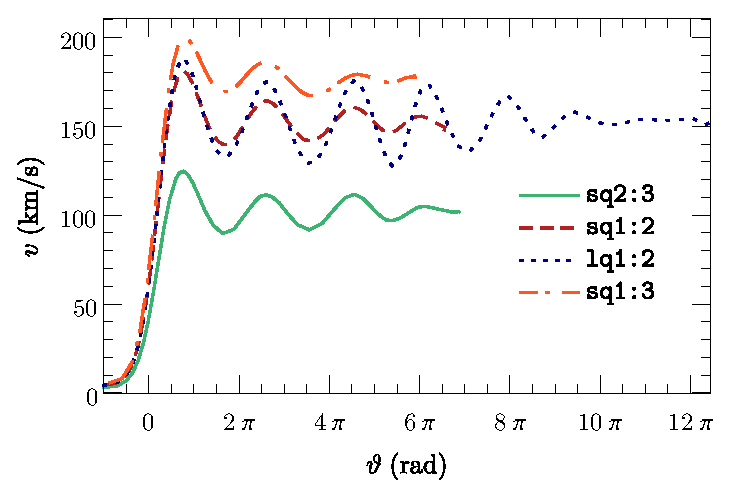
\includegraphics[width=\columnwidth]{kick-theta.eps}}
			}
			\only<+->{
				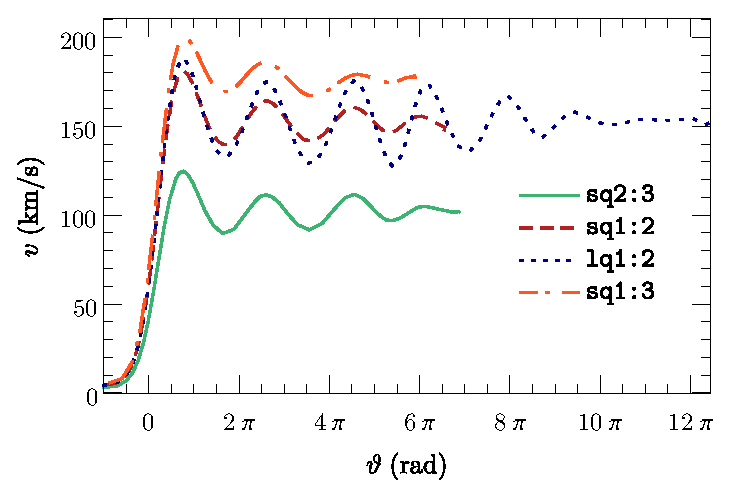
\includegraphics[width=\columnwidth]{kick-theta.eps}
			}
			\vspace{-2 em}
			\begin{itemize}
				\item<+->
					Naively might expect $2\pi$ periodicity...
				\item<+->
					...but we mustn't forget \alert{apsidal precession} 
					(cf. Mercury) which we would expect to 
					slightly decrease the period.
			\end{itemize}
	\end{columns}
\end{frame}

\subsection{Waveform observations}
\begin{frame}{Waveform observations}
	\begin{columns}
		\column{0.45\textwidth}
			\only<.->{
				\centering
				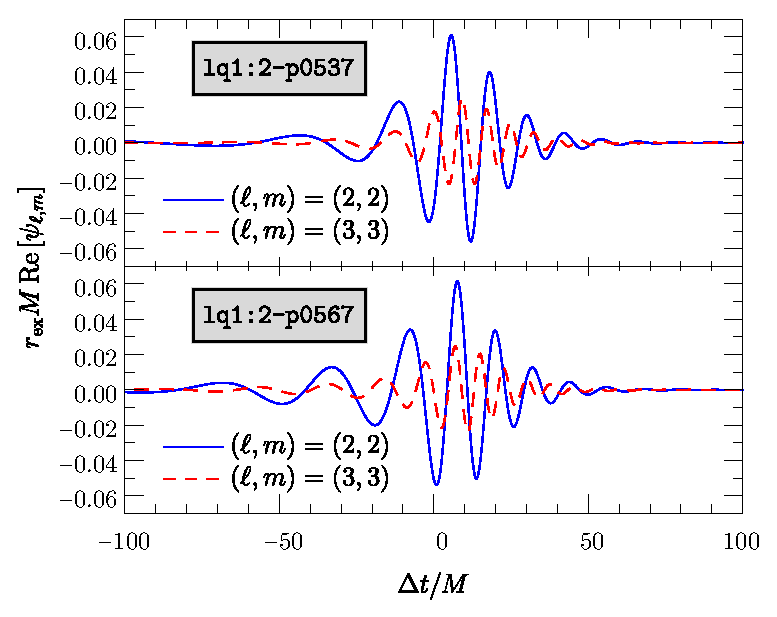
\includegraphics[width=\columnwidth]{mode-kick-extrema.eps}
			}
			\vspace{-1.5em}
			\begin{itemize}
 				\item<.-> Top: $v=128\text{ km/s}$
 				\item<.-> bottom: $v=173\text{ km/s}$
	 		\end{itemize}
		\column{0.55\textwidth}
			\begin{itemize}
				\item<.->
					Unlike for the radiated energy, the radiated momentum
					involves complex (in both senses of the word) 
					\alert{interactions} between different multipoles
					[cf. Eq.~\eqref{eq:P+rad}]
				\item<+->
					On the left, the $(\ell,m)=(2,2)$ and $(3,3)$, 
					modes of $\Psi_4$ are shown for two \alert{consecutive} 
					local extrema on the
					curves $v=v(p)$ for \texttt{lq1:2} ($\Delta t=0$ at common 
					AH formation).
				\item<+->
					The modes appear to be more \alert{in phase} for the 
					bigger kick 
					and more \alert{in antiphase} for the smaller kick.
				\item<+->
					This pattern is observed for other 
					sequences/consecutive extrema.
			\end{itemize}
	\end{columns}
\end{frame}

\section*{Summary}

\begin{frame}{Summary}

  \begin{itemize}
    \item
    	We have evolved 274 BBH configurations with mass ratio 
    	$q=2/3$, $1/2$ and $1/3$ spread across four 
    	sequences with \texttt{GRChombo} and \texttt{Lean}.
    \item
    	We have demonstrated that \texttt{GRChombo} is capable of 
    	evolving BBH inspirals with \alert{comparable accuracy} to a well 
    	established NR code (after some work).
    \item
    	For all sequences, we observe \alert{oscillations} in the kick as a 
    	function of eccentricity with
    	a global maximum at $e\sim0.5$. These oscillations differ
    	from that of the final spin and radiated energy.
    \item
    	We posit that this oscillatory behaviour is due to the change in the
    	\alert{infall direction} relative to the \alert{apo/periapsis}. 
    \item
    	We find that longer inspirals lead to bigger and 
    	more frequent oscillations
    \item
    	We observe shifts in the \alert{phase} of subdominant 
    	multipoles of $\Psi_4$ relative to the dominant $(2,2)$ mode
    	between larger and smaller kicks.
  \end{itemize}
  
\end{frame}

\section*{Any questions?}

\end{document}


